\begin{figure}[ht]
\centering
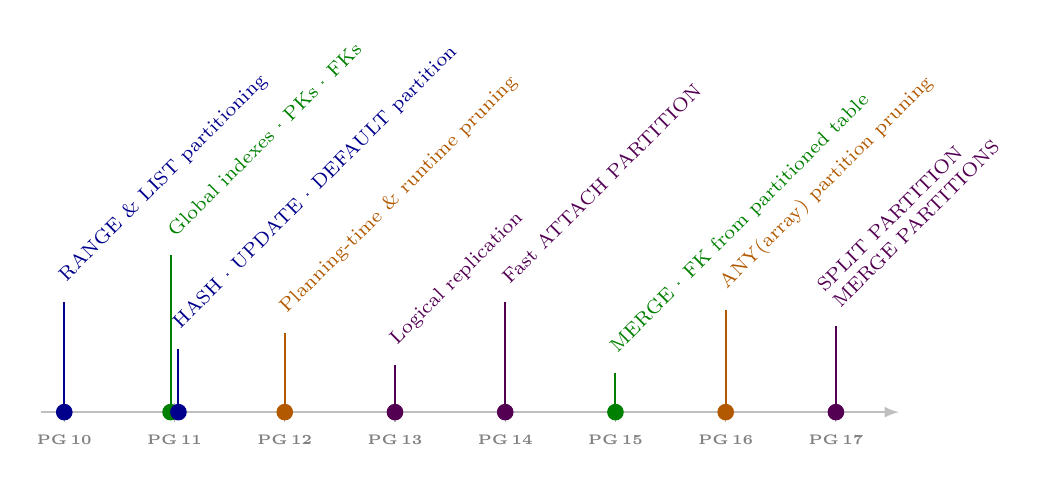
\begin{tikzpicture}[font=\small]

\colorlet{cD}{blue!55!black}
\colorlet{cS}{green!50!black}
\colorlet{cP}{orange!70!black}
\colorlet{cO}{violet!65!black}

\draw[black!25, line width=0.8pt, -latex] (-0.3,0) -- (10.6,0);

\foreach \ver in {10,11,12,13,14,15,16,17} {
  \pgfmathsetmacro{\xpos}{(\ver - 10) * 1.4}
  \draw[black!30, thin] (\xpos,-0.12) -- (\xpos,0.12);
  \node[font=\tiny, black!50, anchor=north] at (\xpos,-0.16) {\textbf{PG\,\ver}};
}

%% PG 10 — RANGE & LIST (h=1.4)
\filldraw[cD] (0,0) circle (2.8pt);
\draw[cD, line width=0.75pt] (0,0) -- (0,1.4);
\node[rotate=45, anchor=south west, font=\scriptsize, cD]
  at (0.06,1.44) {RANGE \& LIST partitioning};

%% PG 11 — structural: global indexes, PKs, FKs (h=2.0)
\filldraw[cS] (1.35,0) circle (2.8pt);
\draw[cS, line width=0.75pt] (1.35,0) -- (1.35,2.0);
\node[rotate=45, anchor=south west, font=\scriptsize, cS]
  at (1.41,2.04) {Global indexes · PKs · FKs};

%% PG 11 — HASH + behavior: UPDATE, DEFAULT (h=0.8)
\filldraw[cD] (1.45,0) circle (2.8pt);
\draw[cD, line width=0.75pt] (1.45,0) -- (1.45,0.8);
\node[rotate=45, anchor=south west, font=\scriptsize, cD]
  at (1.51,0.84) {HASH · UPDATE · DEFAULT partition};

%% PG 12 — planning-time & runtime pruning (h=1.0)
\filldraw[cP] (2.8,0) circle (2.8pt);
\draw[cP, line width=0.75pt] (2.8,0) -- (2.8,1.0);
\node[rotate=45, anchor=south west, font=\scriptsize, cP]
  at (2.86,1.04) {Planning-time \& runtime pruning};

%% PG 13 — logical replication (h=0.6)
\filldraw[cO] (4.2,0) circle (2.8pt);
\draw[cO, line width=0.75pt] (4.2,0) -- (4.2,0.6);
\node[rotate=45, anchor=south west, font=\scriptsize, cO]
  at (4.26,0.64) {Logical replication};

%% PG 14 — fast ATTACH PARTITION (h=1.4)
\filldraw[cO] (5.6,0) circle (2.8pt);
\draw[cO, line width=0.75pt] (5.6,0) -- (5.6,1.4);
\node[rotate=45, anchor=south west, font=\scriptsize, cO]
  at (5.66,1.44) {Fast ATTACH PARTITION};

%% PG 15 — MERGE + FK from partitioned table (h=0.5)
\filldraw[cS] (7.0,0) circle (2.8pt);
\draw[cS, line width=0.75pt] (7.0,0) -- (7.0,0.5);
\node[rotate=45, anchor=south west, font=\scriptsize, cS]
  at (7.06,0.54) {MERGE · FK from partitioned table};

%% PG 16 — ANY(array) partition pruning (h=1.3)
\filldraw[cP] (8.4,0) circle (2.8pt);
\draw[cP, line width=0.75pt] (8.4,0) -- (8.4,1.3);
\node[rotate=45, anchor=south west, font=\scriptsize, cP]
  at (8.46,1.34) {ANY(array) partition pruning};

%% PG 17 — SPLIT PARTITION + MERGE PARTITIONS (h=1.1, two lines)
\filldraw[cO] (9.8,0) circle (2.8pt);
\draw[cO, line width=0.75pt] (9.8,0) -- (9.8,1.1);
\node[rotate=45, anchor=south west, font=\scriptsize, cO, align=left]
  at (9.86,1.14) {SPLIT PARTITION\\MERGE PARTITIONS};

\end{tikzpicture}
\caption{Declarative partitioning milestones, PG\,10–PG\,17.}
\end{figure}
